\chapter{Antecedentes}
\label{chap:antecedentes}

El desarrollo de sistemas de inteligencia artificial capaces de asistir en la evaluación
del lenguaje no puede abordarse sin antes comprender el dominio en el que se inserta,
las herramientas que la comunidad científica y tecnológica ha desarrollado hasta la fecha y las
limitaciones que aún persisten. En el ámbito de la comunicación aumentativa y
alternativa, la distancia entre lo que la tecnología puede ofrecer y lo que los
clínicos necesitan sigue siendo considerable, en particular para el español.

Este capítulo revisa el estado del arte en los campos que confluyen en este trabajo.
En primer lugar se describe el marco clínico: los \textbf{\ac{SAAC}}, las características
lingüísticas del lenguaje que producen sus usuarios y el \textbf{protocolo de Gloria Soto}
(\ac{PAALSS}) que se pretende automatizar. A continuación se analizan las iniciativas
de análisis automático de muestras de lenguaje (\emph{Language Sample Analysis}, LSA),
tanto las herramientas clásicas como las propuestas más recientes basadas en \ac{PLN} y
aprendizaje profundo. Por último, se han revisado las técnicas de aprendizaje con pocos
ejemplos en entornos clínicos, los sistemas de extracción de información, y los avances 
actuales en transcripción automática y diarización de hablantes, elementos todos ellos necesarios para el pipeline propuesto en este trabajo.


%% ============================================================
\section{Sistemas de Comunicación Aumentativa y Alternativa}
\label{sec:saac}
%% ============================================================

Los \ac{SAAC} comprenden cualquier método, estrategia, símbolo o dispositivo que
complementa o reemplaza el habla cuando esta es insuficiente para satisfacer las
necesidades comunicativas de una persona~\cite{nlp_aac_application}.  Sus usuarios
incluyen personas con parálisis cerebral, \ac{TEA}, síndrome de Down, afasia y otras
condiciones que afectan a la producción oral.  Según la tipología habitual, los \ac{SAAC}
pueden ser \emph{sin ayuda} (gestos manuales, signos) o \emph{con ayuda}
(\emph{aided AAC}), siendo estos últimos los que producen el lenguaje asistido que
analiza el protocolo estudiado en este trabajo.

Los sistemas \emph{con ayuda} incluyen tableros de comunicación en papel, tableros
digitales y dispositivos generadores de voz (\emph{Speech-Generating Devices}, \ac{SGD})
controlados mediante pulsadores, seguimiento ocular o pantallas táctiles.  La interfaz de
usuario suele basarse en pictogramas con texto superpuesto. El usuario selecciona los 
símbolos de forma secuencial para construir mensajes, lo que impone una dinámica muy 
diferente a la del habla natural: la velocidad de producción es mucho menor, 
la planificación del enunciado es explícita y la longitud de los mensajes tiende a 
ser corta.


\subsection{Características del lenguaje asistido}
\label{subsec:lenguaje_asistido}

El lenguaje producido con \ac{SAAC} presenta rasgos estructurales que lo diferencian
cualitativamente del habla natural~\cite{nlp_aac_application}. La
Figura~\ref{fig:tablero_arasaac} muestra un ejemplo de tablero de comunicación basado
en el catálogo de pictogramas de \ac{ARASAAC}, en el que cada celda contiene un
símbolo gráfico y su etiqueta en texto, que el usuario selecciona de forma secuencial
para construir su mensaje. Entre los rasgos más estudiados del lenguaje asistido se
encuentran:

\begin{figure}[htbp]
  \centering
  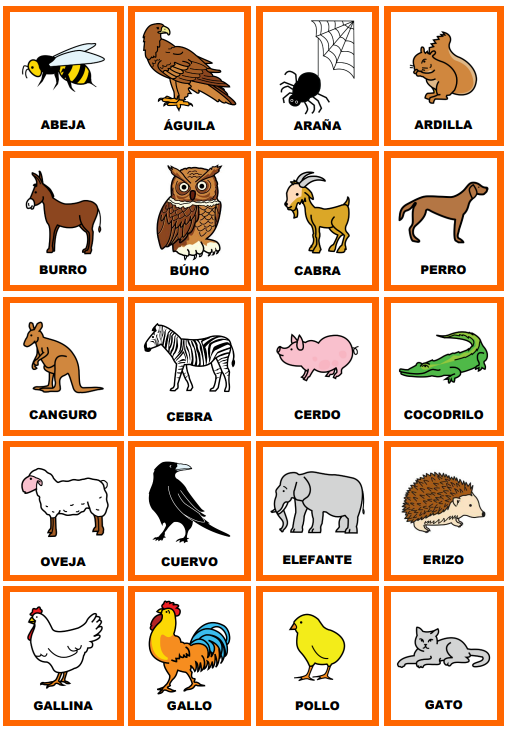
\includegraphics[width=0.4\textwidth]{figs/tablero_arasaac.png}
  \caption{Ejemplo de tablero de comunicación basado en pictogramas \ac{ARASAAC}.
  Fuente: \ac{ARASAAC} (\url{https://arasaac.org})}
  \label{fig:tablero_arasaac}
\end{figure}

\begin{itemize}
  \item \emph{Enunciados telegráficos.} Los usuarios tienden a emitir 
  secuencias reducidas de símbolos omitiendo elementos gramaticales funcionales como 
  artículos, preposiciones o morfemas flexivos.
  \item \emph{Orden de palabras no canónico.} La ausencia de morfología flexiva obliga 
  a interpretar el orden de las palabras. El protocolo de Soto evalúa específicamente 
  la presencia del orden Sujeto-Verbo-Objeto (\ac{SVO}).
  \item \emph{Omisión de morfología gramatical.} Dado que los pictogramas suelen 
  representar formas de cita (infinitivos, sustantivos sin flexión), la concordancia de 
  género, número, tiempo y aspecto puede estar ausente o ser asistida por el propio 
  dispositivo.
  \item \emph{Vocabulario restringido al conjunto disponible.} El léxico accesible depende 
  del vocabulario programado en el dispositivo, lo que puede diferir del vocabulario activo 
  real del usuario y sesgar los análisis basados en diversidad léxica.
\end{itemize}

Estos rasgos implican que los modelos y herramientas de \ac{PLN} entrenados sobre corpus
de habla típica no son directamente aplicables al lenguaje asistido sin adaptación
previa. El lenguaje producido por estos usuarios constituye un tipo de texto distinto al 
habla conversacional estándar, telegráfico y restringido por el vocabulario del dispositivo.
Esta constatación justifica que el sistema propuesto aquí no se limite al canal auditivo sino que
contemple también la información visual del vídeo de la sesión, si es posible.


\subsection{El Protocolo para el Análisis de Muestras de Lenguaje Asistido en SAAC}
\label{subsec:paalss}

El \textbf{\ac{PAALSS}} fue desarrollado por Gloria Soto, investigadora de la 
\emph{San Francisco State University}, como marco sistemático para evaluar el perfil 
lingüístico de personas que utilizan \ac{SAAC}~\cite{soto2020protocolo}. 
Un estudio piloto posterior de la propia autora~\cite{soto2024paalss_pilot} aplicó el 
protocolo de forma manual a una muestra de usuarios hispanohablantes, confirmando su 
viabilidad clínica pero constatando la elevada carga de trabajo del análisis manual, 
lo que refuerza la motivación del presente trabajo. El protocolo aborda el análisis 
desde cuatro dimensiones complementarias, cada una centrada en un nivel lingüístico 
diferente:

\begin{itemize}
  \item \emph{Vocabulario.} Se examina la diversidad léxica a partir de una lista de 219 
  palabras organizadas en categorías (sustantivos, verbos, adjetivos, pronombres y 
  palabras de función). La métrica principal es el número de tipos de palabras distintos 
  (\emph{number of different words}), complementada con la proporción de palabras nuevas 
  que el usuario introduce respecto a las que repite a lo largo de la muestra.

  \item \emph{Morfología.} Se analizan los morfemas gramaticales producidos en las dimensiones
  de género, número, tiempo verbal, aspecto y modo. Para cada morfema se registra si el
  usuario lo produce correctamente, lo omite o lo produce con error, lo que permite trazar 
  un perfil morfológico detallado del usuario.

  \item \emph{Complejidad gramatical.} Esta dimensión clasifica los enunciados en niveles de 
  complejidad creciente: desde palabras aisladas hasta cláusulas subordinadas. La métrica clave 
  es la \textbf{\ac{LME}}, calculada en morfemas o en palabras según la modalidad de análisis.

  \item \emph{Sintaxis.} Se evalúa la presencia y corrección del orden \ac{SVO}, la producción de 
  distintos tipos de oraciones (afirmativas, interrogativas, negativas) y el uso de 
  elementos relacionales como conjunciones o pronombres relativos.
\end{itemize}

Para la recogida de muestras, el protocolo recomienda un mínimo de 50 enunciados por
sesión, obtenidos en contextos naturales de interacción comunicativa.  La unidad de
análisis es el \emph{Communication Turn} (CT), definido como cada contribución que realiza
el usuario durante un turno de conversación.  El protocolo manual requiere que un
especialista en \ac{SAAC} transcriba la sesión, segmente los enunciados, los codifique
según las cuatro dimensiones y calcule las métricas globales.  Este proceso puede
extenderse varias horas por sesión, lo que constituye la principal barrera para su uso
sistemático en la práctica clínica y educativa~\cite{lsa_computer_programs}.


%% ============================================================
\section{Análisis automático de muestras de lenguaje}
\label{sec:lsa_automatico}
%% ============================================================

El análisis de muestras de lenguaje (\emph{Language Sample Analysis}, \ac{LSA}) es el
proceso de recoger, transcribir y cuantificar muestras de habla espontánea para obtener
indicadores objetivos del desarrollo o del perfil lingüístico de una persona. Se
considera el patrón de oro para evaluar las habilidades comunicativas expresivas, ya que
refleja el uso real del lenguaje en contextos naturales con mayor validez que las pruebas 
estandarizadas~\cite{lsa_computer_programs}.


\subsection{Herramientas clásicas: SALT, CLAN y SUGAR}
\label{subsec:salt_clan}

Los tres programas más utilizados en el contexto anglosajón para el LSA clínico: \textbf{\ac{SALT}}
(\emph{Systematic Analysis of Language Transcripts}), \textbf{\ac{CLAN}} (\emph{Computerized Language
Analysis}) y \textbf{\ac{SUGAR}} (\emph{Sampling Utterances and Grammatical Analysis Revised}),
aplicados a dos estudios de caso con niños preescolares \cite{lsa_computer_programs}.

\textbf{\ac{SALT}} es un software que calcula automáticamente métricas de producción lingüística a
partir de transcripciones en su propio formato anotado. Entre las métricas que computa
se incluyen la \ac{LME} en palabras y morfemas, el número de tipos léxicos distintos, la
tasa de disfluencias (\emph{mazes} o la proporción de elementos no fluidos en la producción 
del hablante) y el número de enunciados por minuto, y dispone de bases de datos normativas 
en inglés y español para distintos contextos comunicativos. Sin embargo, exige que el clínico 
proporcione la transcripción ortográfica completa y codifique manualmente las anotaciones 
morfológicas en una sintaxis propia, proceso que requiere formación específica y consume tiempo 
considerable~\cite{lsa_morphological_auto}.

\textbf{\ac{CLAN}} es la herramienta de análisis del sistema \textbf{\ac{CHILDES}} (\emph{Child Language Data
Exchange System}), que utiliza el formato de transcripción \textbf{\ac{CHAT}} (\emph{Codes for the
Human Analysis of Talk}). A diferencia de \ac{SALT}, \ac{CLAN} identifica automáticamente los
morfemas gramaticales con una precisión media del 94\%, sin necesidad de codificación
manual, e incluye módulos para el análisis morfosintáctico que permiten contrastar los resultados 
con \textbf{\ac{KIDEVAL}}, una base de datos normativa derivada de los corpus CHILDES con aproximadamente 
450 niños de desarrollo típico. 

\textbf{\ac{SUGAR}}, por su parte, no es un programa independiente sino un protocolo de codificación 
sobre un procesador de texto convencional: omite la codificación de morfemas y rellenos, lo que lo 
convierte en el más rápido de los tres (entre 18 y 22 minutos de codificación por muestra de 50 enunciados 
en los casos analizados por los autores), a costa de no detectar errores gramaticales ni calcular 
morfemas automáticamente.

Ninguno de los tres programas resulta adecuado para el lenguaje asistido por \ac{SAAC} para 
este proyecto: sus bases de datos normativas se construyeron sobre habla oral de niños con 
desarrollo típico, sin contemplar la ausencia de morfología en los pictogramas, el componente
gestual y multimodal ni el telegrafismo estructural propios del lenguaje
asistido, así como la barrera del idioma, ya que estas base de datos 
solo existen para el inglés y está construida sobre muestras de niños con desarrolo oral típico, 
sin \ac{SAAC} \cite{lsa_computer_programs}. Esta carencia es precisamente la que motivó el desarrollo 
del protocolo \ac{PAALSS} por parte de Gloria Soto.


\subsection{Automatización del pipeline de análisis}
\label{subsec:batchalign}

El trabajo más completo publicado hasta la fecha sobre la automatización integral del
\ac{LSA} es \emph{Batchalign}~\cite{lsa_automation_jslhr}. El sistema encadena siete módulos 
secuenciales:

\begin{enumerate}
  \item \emph{Reconocimiento automático del habla} (\ac{ASR}, \emph{Automatic Speech 
  Recognition}) mediante Rev~AI, con tasas de error de palabra (\emph{Word Error 
  Rate}, \ac{WER}) del 2{,}4--3{,}4\% en habla adulta.
  \item \emph{Segmentación en enunciados} mediante un modelo \ac{BERT} que predice los 
  límites de turno sobre la transcripción en crudo; alcanza una F1 del 86{,}9\%.
  \item \emph{Corrección automática} de la transcripción generada por el \ac{ASR}.
  \item \emph{Identificación de hablantes} o \emph{speaker diarization}.
  \item \emph{Alineación forzada} a nivel de palabra mediante el \emph{Montreal Forced 
  Aligner} (\ac{MFA}), que asigna marcas temporales a cada token.
  \item \emph{Corrección humana} de los errores residuales.
  \item \emph{Análisis morfosintáctico} automático mediante los módulos de \ac{CLAN}.
\end{enumerate}

\emph{Batchalign} reduce el tiempo de transcripción humana en un 75\% respecto al proceso
completamente manual, manteniendo una calidad comparable con la anotación experta. No
obstante, el sistema está diseñado para inglés y corpus de habla típica adulta, por lo
que su transferencia directa a lenguaje asistido en español requiere adaptación
sustancial y validación del proceso.


%% ============================================================
\section{PLN aplicado a lenguaje atípico}
\label{sec:pln_atipico}
%% ============================================================

El \ac{PLN} ha sido aplicado progresivamente al análisis de lenguaje producido en
condiciones no estándar: habla infantil, lenguaje de aprendices de segunda lengua,
habla de personas con trastornos neurológicos y comunicación asistida. Esta sección
revisa los avances más relevantes para este trabajo.


\subsection{Modelos de lenguaje y análisis morfosintáctico en español}
\label{subsec:pln_espanol}

Para el análisis morfosintáctico del español existen varias herramientas de referencia.
\emph{spaCy}~\cite{lsa_swiss_benchmark} ofrece modelos estadísticos y de redes neuronales para
el etiquetado \ac{POS}, el análisis de dependencias y el reconocimiento de entidades.

\emph{BETO}~\cite{beto_morphological} es un modelo tipo \emph{BERT} preentrenado sobre el corpus
\emph{BooksCorpus} en español más la Wikipedia española (3~GB), que ha demostrado mejorar el
rendimiento en tareas de clasificación de secuencias, etiquetado de secuencias y análisis
sintáctico en español respecto a los modelos multilingües.

Para el etiquetado \ac{POS} del habla espontánea en español,~\cite{spoken_spanish_pos}
se publicó COSER-PoS, un conjunto de datos de referencia anotado manualmente sobre
transcripciones de habla oral espontánea que permite evaluar sistemáticamente los
modelos existentes en condiciones de habla no formal, más cercanas al lenguaje asistido
que los corpus de texto escrito.  La evaluación reportada muestra que spaCy alcanza 
una exactitud (\emph{accuracy}) de entre 0{,}90 y 0{,}93 sobre habla oral, 
frente al 0{,}98--0{,}99 que obtienen sobre el corpus \emph{AnCora} de texto escrito,
lo que evidencia una caída de rendimiento sistemática al pasar de texto formal a habla
espontánea.

La naturaleza del lenguaje asistido plantea retos adicionales para estos modelos: 
la ausencia de morfología flexiva, el orden de palabras atípico y el vocabulario
reducido dan lugar a estructuras que se alejan de la distribución estadística de los
corpus de entrenamiento. Esto sugiere la necesidad de estrategias de adaptación al
dominio (\emph{domain adaptation}) o de enfoques con pocos ejemplos (\emph{few-shot}).


\subsection{PLN en contextos clínicos de lenguaje atípico}
\label{subsec:pln_clinico}

La aplicación de \ac{PLN} a la caracterización del lenguaje en poblaciones con trastornos
del neurodesarrollo ha avanzado considerablemente en la última década. Se ha demostrado 
que ciertas métricas lingüísticas calculadas automáticamente sobre transcripciones son 
sensibles a las diferencias en el patrón de lenguaje del \ac{TEA} \cite{nlp_autism_automated}. 
También se pudo demostrar que modelos estadísticos simples entrenados sobre datos clínicos 
limitados pueden replicar con precisión casi perfecta las anotaciones morfológicas de un 
experto \cite{lsa_morphological_auto}.

Se han identificado tres retos específicos del LSA en poblaciones pediátricas \cite{lsa_swiss_benchmark}: 

\begin{enumerate}
  \item La alta variabilidad inter e intrasujeto en pronunciación y vocabulario.
  \item La presencia de estructuras agramaticales o incompletas que confunden los modelos \ac{POS}.
  \item La escasez de datos anotados en habla infantil clínica, que impide el ajuste fino 
  (\emph{fine-tuning}) de modelos grandes
\end{enumerate}


%% ============================================================
\section{Aprendizaje con pocos ejemplos en PLN clínico}
\label{sec:fewshot}
%% ============================================================

Uno de los principales obstáculos para aplicar \ac{PLN} a dominios clínicos
especializados es la \textbf{escasez de datos etiquetados}: las anotaciones requieren
conocimiento experto costoso y tiempo considerable, mientras que las restricciones de
privacidad y la rareza de las condiciones estudiadas limitan la disponibilidad de
\emph{corpus} públicos. En el caso del lenguaje asistido por \ac{SAAC} en español esta
restricción es especialmente severa: no existe ningún corpus anotado
morfosintácticamente de acceso público, y la anotación del protocolo \ac{PAALSS}
requiere un especialista con formación específica en \ac{SAAC}. El aprendizaje con
pocos ejemplos (\emph{few-shot learning}) es la familia de técnicas que aborda
precisamente este escenario, permitiendo aprovechar modelos de lenguaje preentrenados
con una supervisión adicional mínima.

En el caso del lenguaje asistido por \ac{SAAC}, la escasez de datos se agrava por la
naturaleza misma del canal de comunicación: los pictogramas siempre representan la
\textbf{forma de cita} (infinitivo para los verbos, singular para sustantivos y adjetivos),
por lo que la información morfológica flexiva nunca está codificada explícitamente en
el texto producido. El sistema debe inferir, a partir del contexto conversacional, si
una forma como \emph{comer} corresponde a un presente habitual, a un imperativo o a
una referencia temporal pasada. Esta ambigüedad sistemática requiere un clasificador
capaz de operar con un número muy reducido de ejemplos anotados por un especialista
en \ac{SAAC}, lo que sitúa el aprendizaje con pocos ejemplos como la estrategia
natural para este dominio.

En el contexto de los modelos de lenguaje basados en \emph{Transformer}, pueden
distinguirse dos estrategias principales. El \emph{in-context learning} consiste en
incluir directamente en el \emph{prompt} varios ejemplos del formato \textbf{entrada-etiqueta}
y dejar que el modelo infiera el patrón sin actualizar ningún parámetro; esta
estrategia es característica de los modelos generativos de gran escala (\ac{LLM} de
centenares de miles de millones de parámetros) y resulta difícil de aplicar de forma
local por sus requisitos computacionales. Por otro lado, el ajuste fino
(\emph{fine-tuning}) sobre un conjunto reducido de ejemplos puede causar
sobreajuste y degradar las representaciones aprendidas durante el preentrenamiento,
en especial cuando solo se dispone de decenas de instancias por clase. Entre ambos
extremos, los métodos de aprendizaje con pocos ejemplos basados en modelos de lenguaje
enmascarado (\emph{Masked Language Model}, \ac{MLM}) ofrecen un equilibrio adecuado
para dominios clínicos de pequeño volumen.

El modelo \emph{BETO}~\cite{beto_morphological} es un modelo de tipo \emph{BERT}
preentrenado sobre más de 3 GB de texto en español procedentes de la Wikipedia y del
corpus \emph{BooksCorpus}, lo que lo convierte en la referencia para tareas de \ac{PLN}
en español que requieren comprensión morfológica y sintáctica profunda. \emph{BETO} ha
demostrado superar a los modelos multilingües en tareas de clasificación, etiquetado y
análisis sintáctico sobre el español, y resulta especialmente apropiado para el análisis
del lenguaje asistido porque su arquitectura de tipo \ac{MLM} admite la incorporación
de plantillas de clasificación con muy pocos ejemplos.

El método \textbf{\ac{PET}} (\emph{Pattern-Exploiting Training})~\cite{fewshot_clinical_nlp}
reformula la tarea de clasificación como un problema de modelado de lenguaje enmascarado:
dado un texto de entrada, se construye una plantilla (\emph{pattern}) que inserta el
texto en una oración incompleta, y se designa un verbalizador (\emph{verbalizer}) que
mapea las etiquetas de clase a \emph{tokens} concretos del vocabulario del modelo. El modelo
predice el \emph{token} más probable en la posición \texttt{[MASK]} y la clase predicha es la
etiqueta correspondiente al \emph{token} ganador. Este enfoque no requiere modificar la cabeza
de clasificación del modelo: se aprovecha directamente la distribución de probabilidad
del \ac{MLM} sobre el vocabulario del modelo base. Cuando se dispone de varios patrones
alternativos para una misma tarea, los predicciones de cada plantilla se combinan
mediante un proceso de destilación en un clasificador suave, lo que reduce la varianza
debida a la elección de una única plantilla.

Los resultados reportados en un entorno clínico de recursos limitados son altamente relevantes 
para este trabajo~\cite{fewshot_clinical_nlp}: con tan solo 20 ejemplos anotados por clase, 
\ac{PET} aplicado sobre un modelo \emph{BERT} adaptado al dominio médico eleva la precisión 
de la clasificación del 46\% al 79{,}1\% obtenida con un clasificador supervisado convencional 
sobre el mismo número de ejemplos. Esta ganancia de 33 puntos porcentuales con igual volumen de supervisión 
respalda la adopción de \ac{PET} sobre \emph{BETO} para el análisis de las categorías
morfológicas del lenguaje asistido en español, donde el número de ejemplos anotados
disponibles es del mismo orden de magnitud.

Estos resultados se alinean con la observación de Gorman~\cite{lsa_morphological_auto},
en los que se demostró que sistemas de reglas simples pueden superar al aprendizaje
automático supervisado cuando el \emph{corpus} de entrenamiento es reducido, y que la
combinación de reglas con modelos estadísticos permite alcanzar una precisión cercana
a la del anotador experto. Por este motivo, el sistema propuesto en este trabajo adopta
un enfoque híbrido: las categorías morfológicas con criterios explícitos, como la
distinción entre nombre y verbo en pictogramas de función semántica inequívoca, se
resuelven mediante heurísticos basados en el vocabulario \ac{ARASAAC}, reservando
\ac{PET} sobre \emph{BETO} únicamente para las categorías que presentan \textbf{ambigüedad
dependiente del contexto}, como la modalidad verbal o el tiempo gramatical inferido a
partir del enunciado del interlocutor.

%% ============================================================
\section{Generación Aumentada por Recuperación (RAG)}
\label{sec:ia_protocolos}
%% ============================================================

La \textbf{Generación Aumentada por Recuperación} (\ac{RAG}, \emph{Retrieval-Augmented Generation}) es
un paradigma de arquitectura de \ac{IA} generativa que combina un modelo de lenguaje (\ac{LLM}) con
un mecanismo de recuperación de información sobre una colección de documentos externa al
propio modelo. Frente a un \ac{LLM} de propósito general, que responde únicamente a partir
del conocimiento codificado durante su preentrenamiento, un sistema \ac{RAG} ancla cada
respuesta en fragmentos de texto recuperados de un documento concreto, lo que reduce de
forma sustancial las confabulaciones: respuestas plausibles pero incorrectas que mezclan
información de distintas fuentes vistas durante el entrenamiento~\cite{rag_lewis2020}.
Este paradigma resulta especialmente útil en tareas de extracción de información sobre
documentos extensos y de dominio específico, donde la respuesta a una pregunta concreta
existe en el documento pero localizarla manualmente requiere leer y comprender el texto
completo.

La arquitectura de un sistema \ac{RAG} se organiza habitualmente en cuatro fases.
En primer lugar, el documento se segmenta en fragmentos (\emph{chunks}) de tamaño
manejable, normalmente con cierto solapamiento entre fragmentos consecutivos para
preservar el contexto en los límites de cada segmento. A continuación, cada fragmento
se vectoriza mediante un modelo de \emph{embeddings} de frases y se almacena en una
base de datos vectorial que permite la búsqueda eficiente por similitud semántica; en
implementaciones locales se emplea habitualmente \emph{FAISS}
(\emph{Facebook AI Similarity Search}), una biblioteca de código abierto optimizada
para la búsqueda por vecinos más próximos en espacios vectoriales de alta dimensión.
Para cada consulta o campo a rellenar, una etapa de recuperación (\emph{retrieval})
extrae los $k$ fragmentos más similares mediante similitud coseno entre el
\emph{embedding} de la consulta y los del documento. Por último, el \ac{LLM} recibe
un \emph{prompt} estructurado con los fragmentos recuperados como contexto y genera la
respuesta fundamentada exclusivamente en ellos, con la instrucción explícita de señalar
la ausencia de información cuando los fragmentos recuperados no contengan la respuesta.

La viabilidad de esta arquitectura para la extracción de información en protocolos
clínicos ha sido validada empíricamente por Babaeipour~\cite{clinical_nlp_ai_protocol}: en este
estudio se comparó un \ac{LLM} autónomo con un sistema \ac{RAG} sobre la tarea de
extraer información estructurada de protocolos de ensayos clínicos, y el enfoque \ac{RAG}
alcanzó una exactitud del 89\% frente al 62{,}6\% del \ac{LLM} sin recuperación,
reduciendo además de forma sustancial las confabulaciones (\emph{hallucinations}).
Estos resultados confirman que anclar la generación en fragmentos recuperados del
documento de referencia es la estrategia adecuada cuando se requiere que las respuestas
sean trazables y verificables, una propiedad imprescindible en un sistema de asistencia
a la cumplimentación de un protocolo clínico como el \ac{PAALSS}.

En el contexto de este trabajo, la restricción de procesamiento local impuesta por el
\ac{RGPD} descarta el uso de \ac{LLM} accesibles únicamente a través de \ac{API}
externas. La herramienta \emph{Ollama}~\cite{ollama} permite ejecutar localmente
modelos de la familia \emph{Llama} y similares sin ejecutarlos en la nube, ofreciendo una
interfaz de \ac{API} compatible con los estándares habituales de integración, lo que
facilita la sustitución del modelo por versiones más actualizadas a medida que la
investigación avance.


%% ============================================================
\section{Transcripción automática y análisis multimodal}
\label{sec:transcripcion_multimodal}
%% ============================================================

Los avances recientes en reconocimiento automático del habla (\ac{ASR}) y en la
combinación de \ac{ASR} con diarización de hablantes abren la posibilidad de procesar
directamente las grabaciones de vídeo de las sesiones de comunicación asistida.


\subsection{Reconocimiento automático del habla con Whisper}
\label{subsec:whisper}

\emph{Whisper}~\cite{whisper_radford2023} es un modelo \ac{ASR} desarrollado por
\emph{OpenAI} basado en la arquitectura \emph{Transformer encoder-decoder},
preentrenado mediante supervisión débil a gran escala: los 680.000 horas de audio de
entrenamiento proceden de Internet y se emparejan automáticamente con sus
transcripciones en múltiples idiomas, lo que elimina la necesidad de anotación manual
masiva y dota al modelo de una capacidad de generalización notable sobre acentos, ruido
de fondo y registros informales~\cite{whisper_radford2023}. El modelo es capaz de
transcribir y traducir hasta 98 idiomas, incluyendo el español, y supera o iguala el
estado del arte en varios \emph{benchmarks} de robustez sin ajuste fino específico.

El modelo existe en varias configuraciones de tamaño: \texttt{tiny} (39~M parámetros),
\texttt{base} (74~M), \texttt{small} (244~M), \texttt{medium} (769~M) y \texttt{large}
(1.550~M). La variante \texttt{small} ha demostrado ser un compromiso adecuado entre
precisión y coste computacional en aplicaciones de análisis del lenguaje clínico que
requieren despliegue local~\cite{lsa_swiss_benchmark,whisper_diarization_realtime},
mientras que la variante \texttt{large-v3} ofrece la mayor exactitud disponible y
resulta adecuada cuando el equipo dispone de \ac{GPU} con al menos 6~GB de VRAM. Para
el despliegue local eficiente se emplea \texttt{faster-whisper}, una reimplementación
de \emph{Whisper} en \emph{CTranslate2} que reduce el consumo de memoria mediante
cuantización en coma flotante de 16 bits y permite ejecutar el modelo \texttt{large-v3}
en \ac{GPU} con un consumo inferior a 6 GB de VRAM.

Un aspecto relevante para las sesiones de comunicación asistida es que la voz
producida por el dispositivo generador de voz (\ac{TTS}) del comunicador electrónico
difiere acústicamente de la voz humana natural: es más uniforme, sin variaciones de
entonación ni disfluencias. \emph{Whisper} transcribe correctamente los fragmentos de
\ac{TTS}, pero los modelos de diarización pueden tender a asignar estos fragmentos al clúster
del interlocutor adulto en lugar de al usuario del \ac{SAAC}, lo que requiere un
postprocesado específico descrito en el capítulo de metodología.


\subsection{Diarización de hablantes}
\label{subsec:diarizacion}

En las sesiones de comunicación asistida intervienen típicamente al menos dos
participantes: el usuario del \ac{SAAC} y el interlocutor. Para el análisis del protocolo
\ac{PAALSS} es necesario atribuir cada enunciado al hablante correcto, lo que requiere
diarización (\emph{speaker diarization}): la tarea de segmentar el audio y etiquetar cada
segmento con la identidad del hablante.

Existen distintos enfoques para abordar esta tarea. Un primer enfoque combina \emph{Whisper} con
un modelo de \emph{embedding} de hablante y \emph{clustering} incremental sobre los propios
segmentos de la transcripción~\cite{whisper_diarization_realtime}, pensado para
funcionar en tiempo real con un número variable de hablantes, condiciones que no exige el
análisis \ac{PAALSS}, realizado \emph{a posteriori} sobre grabaciones de dos hablantes
fijos. Un segundo enfoque, \textbf{DiCoW} (\emph{Diarization-Conditioned Whisper}),
condiciona el \emph{encoder} de Whisper con la salida de un diarizador externo mediante
máscaras STNO y mecanismos de \emph{Query-Key Biasing} y \emph{Frame-Level
Diarization-Dependent Transformations}~\cite{dicow_diarization}, evitando así el
enrolamiento del hablante objetivo, aunque requiere una etapa externa de diarización y un
ajuste fino sobre corpus en inglés alejados de las condiciones acústicas de una sesión
infantil en español. Un tercer enfoque, \emph{pyannote.audio}~\cite{pyannote_plaquet2023}, es una
herramienta de propósito general que no requiere ajuste fino ni enrolamiento y se
distribuye como \emph{pipeline} preentrenado de uso directo, lo que la hace adecuada
para escenarios fijos de dos hablantes sin restricciones de latencia. Su arquitectura
combina segmentación a nivel de \emph{frame}, extracción de \emph{embeddings} de
hablante y \emph{clustering} jerárquico aglomerativo, y está implementada como
librería Python de código abierto con modelos preentrenados disponibles en
\emph{HuggingFace}.


%% ============================================================
\section{Síntesis comparativa}
\label{sec:comparativa}
%% ============================================================

La revisión realizada en este capítulo pone de manifiesto que los trabajos existentes
abordan componentes aislados del problema pero ninguno integra todos los elementos
necesarios para la automatización del protocolo \ac{PAALSS} en español: la extracción
de enunciados desde vídeo, el procesamiento morfosintáctico del lenguaje asistido, el
cálculo de las métricas del protocolo y el pre-rellenado del formulario clínico. La
Tabla~\ref{tab:comparativa} resume las principales herramientas y enfoques revisados
en relación con las dimensiones más relevantes para este trabajo.

\begin{table}[h]
  \footnotesize
  \renewcommand{\arraystretch}{1.3}
  \setlength{\tabcolsep}{4pt}
  \begin{center}
  \begin{tabular}{|L{2.1cm}|C{1.4cm}|C{1.7cm}|C{1.4cm}|C{1.3cm}|C{1.2cm}|L{4.0cm}|}
  \hline
  \rowcolor{tema!10}
  \bft{Herramienta} & \bft{Idioma} & \bft{Entrada} & \bft{Transcr.\ auto.} & \bft{Morfol.\ auto.} & \bft{Adapt.\ SAAC} & \bft{Limitación principal} \\ \hline
  SALT & EN / ES & Texto manual & No & Parcial & No &
  Requiere transcripción y codificación manual; bases de datos normativas solo en inglés \\ \hline
  CLAN / Batchalign & EN & Texto / Audio & Sí & Sí & No &
  Diseñado para habla oral típica en inglés; no contempla pictogramas ni lenguaje telegráfico \\ \hline
  SUGAR & EN & Texto manual & No & No & No &
  Método manual simplificado; no detecta errores gramaticales ni calcula morfemas \\ \hline
  LLUNA & EN & Texto manual & No & Parcial & No &
  Limitado a narrativas; sin componente multimodal ni adaptación al español \\ \hline
  Medidas LSA/TEA & EN & Texto manual & No & Sí & No &
  Diseñado para \ac{TEA}; no adaptado a \ac{SAAC} ni al español \\ \hline
  Benchmark PLN infantil & DE/FR/\,IT & Texto & No & Sí & No &
  Habla infantil típica en lenguas suizas; sin canal de vídeo ni lenguaje asistido \\ \hline
  \rowcolor{tema!10}
  \bft{Este trabajo} & \bft{ES} & \bft{Vídeo} & \bft{Sí} & \bft{Sí} & \bft{Sí} &
  Validado sobre una única usuaria; canal visual (pictogramas) pendiente de implementar \\ \hline
  \end{tabular}
  \end{center}
  \caption[Comparativa de herramientas]{Comparativa de herramientas y enfoques de análisis automático del lenguaje.}
  \label{tab:comparativa}
  \renewcommand{\arraystretch}{1}
\end{table}

De la comparativa se extraen tres conclusiones que fundamentan las decisiones de diseño
del sistema propuesto. En primer lugar, todas las herramientas existentes para el
\ac{LSA} automático operan sobre texto ya transcrito, sin abordar la extracción de
enunciados desde vídeo, lo que constituye la diferencia más radical del presente
trabajo. En segundo lugar, ninguna herramienta revisada ha sido diseñada o adaptada
para el lenguaje asistido por \ac{SAAC}, lo que implica que las métricas calculadas
sobre habla oral típica no son directamente transferibles. En tercer lugar, la barrera
del idioma es un obstáculo transversal: todos los sistemas con automatización completa
están diseñados y validados para el inglés, lo que justifica la elección de modelos
específicos para el español como \emph{BETO} y \texttt{es\_core\_news\_lg} y la
restricción del alcance del trabajo a una única lengua.
